% Options for packages loaded elsewhere
\PassOptionsToPackage{unicode}{hyperref}
\PassOptionsToPackage{hyphens}{url}
\PassOptionsToPackage{dvipsnames,svgnames,x11names}{xcolor}
%
\documentclass[
  super,
  preprint,
  3p]{elsarticle}

\usepackage{amsmath,amssymb}
\usepackage{lmodern}
\usepackage{iftex}
\ifPDFTeX
  \usepackage[T1]{fontenc}
  \usepackage[utf8]{inputenc}
  \usepackage{textcomp} % provide euro and other symbols
\else % if luatex or xetex
  \usepackage{unicode-math}
  \defaultfontfeatures{Scale=MatchLowercase}
  \defaultfontfeatures[\rmfamily]{Ligatures=TeX,Scale=1}
\fi
% Use upquote if available, for straight quotes in verbatim environments
\IfFileExists{upquote.sty}{\usepackage{upquote}}{}
\IfFileExists{microtype.sty}{% use microtype if available
  \usepackage[]{microtype}
  \UseMicrotypeSet[protrusion]{basicmath} % disable protrusion for tt fonts
}{}
\makeatletter
\@ifundefined{KOMAClassName}{% if non-KOMA class
  \IfFileExists{parskip.sty}{%
    \usepackage{parskip}
  }{% else
    \setlength{\parindent}{0pt}
    \setlength{\parskip}{6pt plus 2pt minus 1pt}}
}{% if KOMA class
  \KOMAoptions{parskip=half}}
\makeatother
\usepackage{xcolor}
\setlength{\emergencystretch}{3em} % prevent overfull lines
\setcounter{secnumdepth}{5}
% Make \paragraph and \subparagraph free-standing
\ifx\paragraph\undefined\else
  \let\oldparagraph\paragraph
  \renewcommand{\paragraph}[1]{\oldparagraph{#1}\mbox{}}
\fi
\ifx\subparagraph\undefined\else
  \let\oldsubparagraph\subparagraph
  \renewcommand{\subparagraph}[1]{\oldsubparagraph{#1}\mbox{}}
\fi

\usepackage{color}
\usepackage{fancyvrb}
\newcommand{\VerbBar}{|}
\newcommand{\VERB}{\Verb[commandchars=\\\{\}]}
\DefineVerbatimEnvironment{Highlighting}{Verbatim}{commandchars=\\\{\}}
% Add ',fontsize=\small' for more characters per line
\usepackage{framed}
\definecolor{shadecolor}{RGB}{241,243,245}
\newenvironment{Shaded}{\begin{snugshade}}{\end{snugshade}}
\newcommand{\AlertTok}[1]{\textcolor[rgb]{0.68,0.00,0.00}{#1}}
\newcommand{\AnnotationTok}[1]{\textcolor[rgb]{0.37,0.37,0.37}{#1}}
\newcommand{\AttributeTok}[1]{\textcolor[rgb]{0.40,0.45,0.13}{#1}}
\newcommand{\BaseNTok}[1]{\textcolor[rgb]{0.68,0.00,0.00}{#1}}
\newcommand{\BuiltInTok}[1]{\textcolor[rgb]{0.00,0.23,0.31}{#1}}
\newcommand{\CharTok}[1]{\textcolor[rgb]{0.13,0.47,0.30}{#1}}
\newcommand{\CommentTok}[1]{\textcolor[rgb]{0.37,0.37,0.37}{#1}}
\newcommand{\CommentVarTok}[1]{\textcolor[rgb]{0.37,0.37,0.37}{\textit{#1}}}
\newcommand{\ConstantTok}[1]{\textcolor[rgb]{0.56,0.35,0.01}{#1}}
\newcommand{\ControlFlowTok}[1]{\textcolor[rgb]{0.00,0.23,0.31}{#1}}
\newcommand{\DataTypeTok}[1]{\textcolor[rgb]{0.68,0.00,0.00}{#1}}
\newcommand{\DecValTok}[1]{\textcolor[rgb]{0.68,0.00,0.00}{#1}}
\newcommand{\DocumentationTok}[1]{\textcolor[rgb]{0.37,0.37,0.37}{\textit{#1}}}
\newcommand{\ErrorTok}[1]{\textcolor[rgb]{0.68,0.00,0.00}{#1}}
\newcommand{\ExtensionTok}[1]{\textcolor[rgb]{0.00,0.23,0.31}{#1}}
\newcommand{\FloatTok}[1]{\textcolor[rgb]{0.68,0.00,0.00}{#1}}
\newcommand{\FunctionTok}[1]{\textcolor[rgb]{0.28,0.35,0.67}{#1}}
\newcommand{\ImportTok}[1]{\textcolor[rgb]{0.00,0.46,0.62}{#1}}
\newcommand{\InformationTok}[1]{\textcolor[rgb]{0.37,0.37,0.37}{#1}}
\newcommand{\KeywordTok}[1]{\textcolor[rgb]{0.00,0.23,0.31}{#1}}
\newcommand{\NormalTok}[1]{\textcolor[rgb]{0.00,0.23,0.31}{#1}}
\newcommand{\OperatorTok}[1]{\textcolor[rgb]{0.37,0.37,0.37}{#1}}
\newcommand{\OtherTok}[1]{\textcolor[rgb]{0.00,0.23,0.31}{#1}}
\newcommand{\PreprocessorTok}[1]{\textcolor[rgb]{0.68,0.00,0.00}{#1}}
\newcommand{\RegionMarkerTok}[1]{\textcolor[rgb]{0.00,0.23,0.31}{#1}}
\newcommand{\SpecialCharTok}[1]{\textcolor[rgb]{0.37,0.37,0.37}{#1}}
\newcommand{\SpecialStringTok}[1]{\textcolor[rgb]{0.13,0.47,0.30}{#1}}
\newcommand{\StringTok}[1]{\textcolor[rgb]{0.13,0.47,0.30}{#1}}
\newcommand{\VariableTok}[1]{\textcolor[rgb]{0.07,0.07,0.07}{#1}}
\newcommand{\VerbatimStringTok}[1]{\textcolor[rgb]{0.13,0.47,0.30}{#1}}
\newcommand{\WarningTok}[1]{\textcolor[rgb]{0.37,0.37,0.37}{\textit{#1}}}

\providecommand{\tightlist}{%
  \setlength{\itemsep}{0pt}\setlength{\parskip}{0pt}}\usepackage{longtable,booktabs,array}
\usepackage{calc} % for calculating minipage widths
% Correct order of tables after \paragraph or \subparagraph
\usepackage{etoolbox}
\makeatletter
\patchcmd\longtable{\par}{\if@noskipsec\mbox{}\fi\par}{}{}
\makeatother
% Allow footnotes in longtable head/foot
\IfFileExists{footnotehyper.sty}{\usepackage{footnotehyper}}{\usepackage{footnote}}
\makesavenoteenv{longtable}
\usepackage{graphicx}
\makeatletter
\def\maxwidth{\ifdim\Gin@nat@width>\linewidth\linewidth\else\Gin@nat@width\fi}
\def\maxheight{\ifdim\Gin@nat@height>\textheight\textheight\else\Gin@nat@height\fi}
\makeatother
% Scale images if necessary, so that they will not overflow the page
% margins by default, and it is still possible to overwrite the defaults
% using explicit options in \includegraphics[width, height, ...]{}
\setkeys{Gin}{width=\maxwidth,height=\maxheight,keepaspectratio}
% Set default figure placement to htbp
\makeatletter
\def\fps@figure{htbp}
\makeatother
\newlength{\cslhangindent}
\setlength{\cslhangindent}{1.5em}
\newlength{\csllabelwidth}
\setlength{\csllabelwidth}{3em}
\newlength{\cslentryspacingunit} % times entry-spacing
\setlength{\cslentryspacingunit}{\parskip}
\newenvironment{CSLReferences}[2] % #1 hanging-ident, #2 entry spacing
 {% don't indent paragraphs
  \setlength{\parindent}{0pt}
  % turn on hanging indent if param 1 is 1
  \ifodd #1
  \let\oldpar\par
  \def\par{\hangindent=\cslhangindent\oldpar}
  \fi
  % set entry spacing
  \setlength{\parskip}{#2\cslentryspacingunit}
 }%
 {}
\usepackage{calc}
\newcommand{\CSLBlock}[1]{#1\hfill\break}
\newcommand{\CSLLeftMargin}[1]{\parbox[t]{\csllabelwidth}{#1}}
\newcommand{\CSLRightInline}[1]{\parbox[t]{\linewidth - \csllabelwidth}{#1}\break}
\newcommand{\CSLIndent}[1]{\hspace{\cslhangindent}#1}

\makeatletter
\makeatother
\makeatletter
\makeatother
\makeatletter
\@ifpackageloaded{caption}{}{\usepackage{caption}}
\AtBeginDocument{%
\ifdefined\contentsname
  \renewcommand*\contentsname{Table of contents}
\else
  \newcommand\contentsname{Table of contents}
\fi
\ifdefined\listfigurename
  \renewcommand*\listfigurename{List of Figures}
\else
  \newcommand\listfigurename{List of Figures}
\fi
\ifdefined\listtablename
  \renewcommand*\listtablename{List of Tables}
\else
  \newcommand\listtablename{List of Tables}
\fi
\ifdefined\figurename
  \renewcommand*\figurename{Figure}
\else
  \newcommand\figurename{Figure}
\fi
\ifdefined\tablename
  \renewcommand*\tablename{Table}
\else
  \newcommand\tablename{Table}
\fi
}
\@ifpackageloaded{float}{}{\usepackage{float}}
\floatstyle{ruled}
\@ifundefined{c@chapter}{\newfloat{codelisting}{h}{lop}}{\newfloat{codelisting}{h}{lop}[chapter]}
\floatname{codelisting}{Listing}
\newcommand*\listoflistings{\listof{codelisting}{List of Listings}}
\makeatother
\makeatletter
\@ifpackageloaded{caption}{}{\usepackage{caption}}
\@ifpackageloaded{subcaption}{}{\usepackage{subcaption}}
\makeatother
\makeatletter
\@ifpackageloaded{tcolorbox}{}{\usepackage[many]{tcolorbox}}
\makeatother
\makeatletter
\@ifundefined{shadecolor}{\definecolor{shadecolor}{rgb}{.97, .97, .97}}
\makeatother
\makeatletter
\makeatother
\journal{Journal Name}
\makeatletter
\@ifpackageloaded{tikz}{}{\usepackage{tikz}}
\makeatother
        \newcommand*\circled[1]{\tikz[baseline=(char.base)]{
          \node[shape=circle,draw,inner sep=1pt] (char) {{\scriptsize#1}};}}  
                  
\ifLuaTeX
  \usepackage{selnolig}  % disable illegal ligatures
\fi
\usepackage[]{natbib}
\bibliographystyle{elsarticle-num}
\IfFileExists{bookmark.sty}{\usepackage{bookmark}}{\usepackage{hyperref}}
\IfFileExists{xurl.sty}{\usepackage{xurl}}{} % add URL line breaks if available
\urlstyle{same} % disable monospaced font for URLs
\hypersetup{
  pdftitle={Short Paper},
  pdfauthor={Alice Anonymous; Bob Security; Cat Memes; Derek Zoolander},
  pdfkeywords={keyword1, keyword2},
  colorlinks=true,
  linkcolor={blue},
  filecolor={Maroon},
  citecolor={Blue},
  urlcolor={Blue},
  pdfcreator={LaTeX via pandoc}}

\setlength{\parindent}{6pt}
\begin{document}

\begin{frontmatter}
\title{Short Paper \\\large{A Short Subtitle} }
\author[1]{Alice Anonymous%
\corref{cor1}%
\fnref{fn1}}
 \ead{alice@example.com} 
\author[2]{Bob Security%
%
\fnref{fn2}}
 \ead{bob@example.com} 
\author[2]{Cat Memes%
%
\fnref{fn3}}
 \ead{cat@example.com} 
\author[]{Derek Zoolander%
%
}
 \ead{derek@example.com} 

\affiliation[1]{organization={Some Institute of Technology, Department
Name},addressline={Street Address},city={City},postcode={Postal
Code},postcodesep={}}
\affiliation[2]{organization={Another University, Department
Name},addressline={Street Address},city={City},postcode={Postal
Code},postcodesep={}}

\cortext[cor1]{Corresponding author}
\fntext[fn1]{This is the first author footnote.}
\fntext[fn2]{Another author footnote, this is a very long footnote and
it should be a really long footnote. But this footnote is not yet
sufficiently long enough to make two lines of footnote text.}
\fntext[fn3]{Yet another author footnote.}

        





\begin{keyword}
    keyword1 \sep 
    keyword2
\end{keyword}
\end{frontmatter}
    \ifdefined\Shaded\renewenvironment{Shaded}{\begin{tcolorbox}[borderline west={3pt}{0pt}{shadecolor}, sharp corners, boxrule=0pt, enhanced, breakable, interior hidden, frame hidden]}{\end{tcolorbox}}\fi

Keywords: keyword1, keyword2

Highlights: These are the highlights.

\hypertarget{abstract}{%
\section{Abstract}\label{abstract}}

\hypertarget{background}{%
\subsection{Background}\label{background}}

Deserunt voluptate cupidatat officia mollit magna irure nisi. Mollit
adipisicing fugiat laboris sunt ex incididunt reprehenderit. Et velit
anim est minim ad esse excepteur officia Lorem nulla cillum est. Tempor
Lorem eu aliqua mollit et dolor.

\hypertarget{methods}{%
\subsection{Methods}\label{methods}}

Eu eu nostrud cillum duis aliquip ad do eu quis anim nostrud magna
consectetur reprehenderit ad. Pariatur adipisicing commodo velit et ut
incididunt deserunt in. Enim sint voluptate officia. Nostrud occaecat
irure qui velit tempor irure veniam nostrud enim amet labore anim.

\hypertarget{results}{%
\subsection{Results}\label{results}}

Irure enim duis pariatur magna incididunt exercitation magna ad eiusmod
aliqua do sint exercitation. Sint ea ex amet sunt sint fugiat proident
aliqua duis exercitation excepteur sit dolor. Pariatur amet Lorem ex
aliqua duis anim proident. Ad qui enim exercitation et qui nostrud velit
ad deserunt dolore occaecat do.

\hypertarget{discussion}{%
\subsection{Discussion}\label{discussion}}

Sint ad ut tempor aliqua laborum eiusmod. Sint labore nulla cillum
pariatur sit eiusmod adipisicing est ex ex irure incididunt amet et in.
Tempor ut ut velit irure ipsum do. Dolore veniam eu sit elit laborum
officia reprehenderit voluptate ut dolore.

\newpage{}

\hypertarget{introduction}{%
\section{Introduction}\label{introduction}}

Here is a citation \citep{Marwick2017}.

\hypertarget{methods-1}{%
\section{Methods}\label{methods-1}}

\hypertarget{participants}{%
\subsection{Participants}\label{participants}}

\hypertarget{measures}{%
\subsection{Measures}\label{measures}}

\hypertarget{analytical-strategy}{%
\subsection{Analytical Strategy}\label{analytical-strategy}}

\hypertarget{results-1}{%
\section{Results}\label{results-1}}

\begin{Shaded}
\begin{Highlighting}[]
\CommentTok{\# Note the path that we need to use to access our data files when rendering this document}
\NormalTok{my\_data }\OtherTok{\textless{}{-}} \FunctionTok{read.csv}\NormalTok{(here}\SpecialCharTok{::}\FunctionTok{here}\NormalTok{(}\StringTok{\textquotesingle{}src/data/raw\_data/my\_csv\_file.csv\textquotesingle{}}\NormalTok{))}
\end{Highlighting}
\end{Shaded}

\begin{Shaded}
\begin{Highlighting}[]
\FunctionTok{plot}\NormalTok{(}\FunctionTok{rnorm}\NormalTok{(}\DecValTok{10}\NormalTok{))}
\end{Highlighting}
\end{Shaded}

\begin{figure}[H]

{\centering 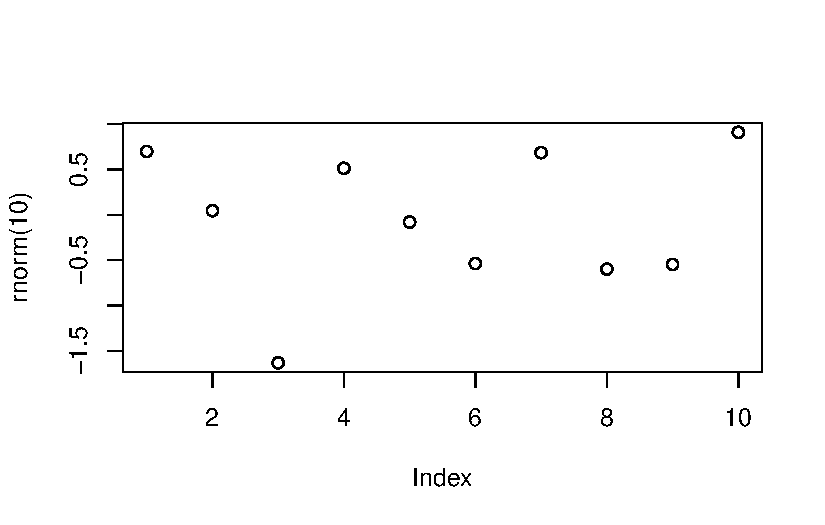
\includegraphics{index_files/figure-pdf/fig-demo-plot-1.pdf}

}

\caption{\label{fig-demo-plot}A plot of random numbers}

\end{figure}

Figure Figure~\ref{fig-demo-plot} shows how we can have a caption and
cross-reference for a plot. Note that figure label and cross-references
must both be prefixed with \texttt{fig-}

Here is an example of inline code 3.14 in the middle of a sentence.

Here is an example of inline code 3.14 in the middle of a sentence.

\hypertarget{discussion-1}{%
\section{Discussion}\label{discussion-1}}

\hypertarget{acknowledgements}{%
\section{Acknowledgements}\label{acknowledgements}}

\hypertarget{references}{%
\section{References}\label{references}}

\hypertarget{refs}{}
\begin{CSLReferences}{0}{0}
\end{CSLReferences}

\newpage

\hypertarget{refs}{}
\begin{CSLReferences}{0}{0}
\end{CSLReferences}

\hypertarget{colophon}{%
\subsubsection{Colophon}\label{colophon}}

This report was generated on 2023-01-18 10:33:20 using the following
computational environment and dependencies:

\begin{Shaded}
\begin{Highlighting}[]
\CommentTok{\# which R packages and versions?}
\ControlFlowTok{if}\NormalTok{ (}\StringTok{"devtools"} \SpecialCharTok{\%in\%} \FunctionTok{installed.packages}\NormalTok{()) devtools}\SpecialCharTok{::}\FunctionTok{session\_info}\NormalTok{()}
\end{Highlighting}
\end{Shaded}

\begin{verbatim}
- Session info ---------------------------------------------------------------
 setting  value
 version  R version 4.2.2 Patched (2023-01-06 r83584)
 os       macOS Big Sur ... 10.16
 system   x86_64, darwin17.0
 ui       X11
 language (EN)
 collate  en_US.UTF-8
 ctype    en_US.UTF-8
 tz       America/Los_Angeles
 date     2023-01-18
 pandoc   2.19.2 @ /usr/local/bin/ (via rmarkdown)

- Packages -------------------------------------------------------------------
 ! package     * version     date (UTC) lib source
 P cachem        1.0.6.9000  2022-11-30 [?] https://r-lib.r-universe.dev (R 4.2.2)
 P callr         3.7.3.9000  2022-12-24 [?] https://r-lib.r-universe.dev (R 4.2.2)
 P cli           3.6.0.9000  2023-01-11 [?] https://r-lib.r-universe.dev (R 4.2.2)
 P collapse    * 1.9.0       2023-01-15 [?] CRAN (R 4.2.0)
 P colorspace    2.1-0       2022-12-13 [?] https://r-forge.r-universe.dev (R 4.2.2)
 P crayon        1.5.2       2022-09-29 [?] CRAN (R 4.2.0)
 P data.table  * 1.14.6      2022-11-16 [?] CRAN (R 4.2.0)
 P devtools      2.4.5.9000  2022-10-11 [?] https://r-lib.r-universe.dev (R 4.2.1)
 P digest        0.6.31      2022-12-11 [?] CRAN (R 4.2.0)
 P dplyr       * 1.0.99.9000 2023-01-04 [?] repository (https://github.com/tidyverse/dplyr@dbda0c7)
 P ellipsis      0.3.2.9000  2022-12-11 [?] https://r-lib.r-universe.dev (R 4.2.2)
 P evaluate      0.20.1      2023-01-17 [?] https://r-lib.r-universe.dev (R 4.2.2)
 P fansi         1.0.3       2022-03-24 [?] CRAN (R 4.2.0)
 P fastmap       1.1.0.9000  2022-12-23 [?] https://r-lib.r-universe.dev (R 4.2.2)
 P fastverse   * 0.3.0       2022-11-15 [?] CRAN (R 4.2.0)
 P forcats     * 0.5.2.9000  2023-01-10 [?] repository (https://github.com/tidyverse/forcats@bd319e0)
 P fs            1.5.2.9000  2022-12-21 [?] https://r-lib.r-universe.dev (R 4.2.2)
 P generics      0.1.3.9000  2023-01-01 [?] https://r-lib.r-universe.dev (R 4.2.2)
 P ggplot2     * 3.4.0.9000  2023-01-06 [?] https://tidyverse.r-universe.dev (R 4.2.2)
 P glue          1.6.2.9000  2022-12-18 [?] https://tidyverse.r-universe.dev (R 4.2.2)
 P gtable        0.3.1.9000  2022-12-24 [?] https://r-lib.r-universe.dev (R 4.2.2)
 P hms           1.1.2.9002  2022-12-30 [?] https://tidyverse.r-universe.dev (R 4.2.2)
 P htmltools     0.5.4.9000  2023-01-03 [?] https://rstudio.r-universe.dev (R 4.2.2)
 P htmlwidgets   1.6.1       2023-01-07 [?] CRAN (R 4.2.0)
 P httpuv        1.6.8.9000  2023-01-12 [?] https://rstudio.r-universe.dev (R 4.2.2)
 P jsonlite      1.8.4       2022-12-06 [?] CRAN (R 4.2.0)
 P kit         * 0.0.12      2022-10-26 [?] CRAN (R 4.2.0)
 P knitr         1.41.9      2023-01-06 [?] https://yihui.r-universe.dev (R 4.2.2)
 P later         1.3.0.9000  2023-01-10 [?] https://r-lib.r-universe.dev (R 4.2.2)
 P lifecycle     1.0.3.9000  2023-01-05 [?] https://r-lib.r-universe.dev (R 4.2.2)
 P lubridate   * 1.9.0.9000  2022-12-12 [?] https://ropensci.r-universe.dev (R 4.2.2)
 P magrittr    * 2.0.3.9000  2022-12-25 [?] https://tidyverse.r-universe.dev (R 4.2.2)
 P memoise       2.0.1.9000  2023-01-03 [?] https://r-lib.r-universe.dev (R 4.2.2)
 P mime          0.12.1      2022-12-18 [?] https://yihui.r-universe.dev (R 4.2.2)
 P miniUI        0.1.1.1     2018-05-18 [?] CRAN (R 4.2.0)
 P munsell       0.5.0       2018-06-12 [?] CRAN (R 4.2.0)
 P pillar        1.8.1.9006  2023-01-01 [?] https://r-lib.r-universe.dev (R 4.2.2)
 P pkgbuild      1.4.0.9000  2022-11-27 [?] https://r-lib.r-universe.dev (R 4.2.2)
 P pkgconfig     2.0.3       2019-09-22 [?] CRAN (R 4.2.0)
 P pkgload       1.3.2.9000  2022-11-16 [?] https://r-lib.r-universe.dev (R 4.2.2)
 P prettyunits   1.1.1.9000  2022-11-30 [?] https://r-lib.r-universe.dev (R 4.2.2)
 P processx      3.8.0.9000  2022-12-18 [?] https://r-lib.r-universe.dev (R 4.2.2)
 P profvis       0.3.7.9000  2022-04-27 [?] https://rstudio.r-universe.dev (R 4.2.0)
 P promises      1.2.0.9000  2022-04-28 [?] https://rstudio.r-universe.dev (R 4.2.0)
 P ps            1.7.2.9000  2022-12-26 [?] https://r-lib.r-universe.dev (R 4.2.2)
 P purrr       * 1.0.1.9000  2023-01-10 [?] https://tidyverse.r-universe.dev (R 4.2.2)
 P R6            2.5.1.9000  2022-12-27 [?] https://r-lib.r-universe.dev (R 4.2.2)
 P Rcpp          1.0.9       2022-07-08 [?] CRAN (R 4.2.0)
 P readr       * 2.1.3.9000  2022-12-11 [?] https://tidyverse.r-universe.dev (R 4.2.2)
 P remotes       2.4.2       2021-11-30 [?] CRAN (R 4.2.0)
   renv          0.16.0-53   2023-01-13 [1] https://rstudio.r-universe.dev (R 4.2.2)
 P rlang         1.0.6.9000  2022-12-17 [?] https://r-lib.r-universe.dev (R 4.2.2)
 P rmarkdown     2.19.2      2022-12-22 [?] Github (rstudio/rmarkdown@8fabad0)
 P scales        1.2.1.9000  2023-01-01 [?] https://r-lib.r-universe.dev (R 4.2.2)
 P sessioninfo   1.2.2.9000  2022-05-14 [?] https://r~
 P shiny         1.7.4.9001  2023-01-06 [?] https://rstudio.r-universe.dev (R 4.2.2)
 P stringi       1.7.12      2023-01-11 [?] CRAN (R 4.2.2)
 P stringr     * 1.5.0.9000  2022-12-07 [?] https://tidyverse.r-universe.dev (R 4.2.2)
 P tibble      * 3.1.8.9004  2022-12-30 [?] https://tidyverse.r-universe.dev (R 4.2.2)
 P tidyr       * 1.2.1.9001  2023-01-10 [?] repository (https://github.com/tidyverse/tidyr@9174795)
 P tidyselect    1.2.0.9000  2023-01-09 [?] https://r-lib.r-universe.dev (R 4.2.2)
 P tidyverse   * 1.3.2.9000  2023-01-05 [?] repository (https://github.com/tidyverse/tidyverse@3be8283)
 P timechange    0.2.0       2023-01-11 [?] CRAN (R 4.2.0)
 P tzdb          0.3.0.9000  2023-01-04 [?] https://r-lib.r-universe.dev (R 4.2.2)
 P urlchecker    1.0.1.9000  2022-05-14 [?] https://r~
 P usethis       2.1.6.9000  2022-12-13 [?] Github (r-lib/usethis@a98a0e6)
 P utf8          1.2.2       2021-07-24 [?] CRAN (R 4.2.0)
 P vctrs         0.5.1.9000  2023-01-09 [?] Github (r-lib/vctrs@4c57418)
 P withr         2.5.0.9000  2022-12-26 [?] https://r-lib.r-universe.dev (R 4.2.2)
 P xfun          0.36.1      2023-01-12 [?] https://yihui.r-universe.dev (R 4.2.2)
 P xtable        1.8-6       2022-04-14 [?] https://r-forge.r-universe.dev (R 4.2.0)
 P yaml          2.3.6       2022-10-18 [?] CRAN (R 4.2.0)

 [1] /Users/joey/.renv/library/rrtools-8440cc86/R-4.2/x86_64-apple-darwin17.0
 [2] /Users/joey/dev/rrtools/renv/sandbox/R-4.2/x86_64-apple-darwin17.0/84ba8b13

 P -- Loaded and on-disk path mismatch.

------------------------------------------------------------------------------
\end{verbatim}

The current Git commit details are:

\begin{Shaded}
\begin{Highlighting}[]
\CommentTok{\# what commit is this file at? }
\ControlFlowTok{if}\NormalTok{ (}\StringTok{"git2r"} \SpecialCharTok{\%in\%} \FunctionTok{installed.packages}\NormalTok{() }\SpecialCharTok{\&}\NormalTok{ git2r}\SpecialCharTok{::}\FunctionTok{in\_repository}\NormalTok{(}\AttributeTok{path =} \StringTok{"."}\NormalTok{)) git2r}\SpecialCharTok{::}\FunctionTok{repository}\NormalTok{(here}\SpecialCharTok{::}\FunctionTok{here}\NormalTok{())  }
\end{Highlighting}
\end{Shaded}

\begin{verbatim}
Local:    main /Users/joey/dev/rrtools
Remote:   main @ origin (https://github.com/brainworkup/rrtools.git)
Head:     [0467987] 2023-01-18: WORKING somewhat
\end{verbatim}


  \bibliography{src/bib/references.bib,src/bib/bibliography.bib}


\end{document}
